\documentclass[tikz,border=5]{standalone}

\usepackage{mathdots}

\usetikzlibrary{calc}
\usetikzlibrary{decorations.pathreplacing}
\usetikzlibrary{scopes}

\begin{document}
  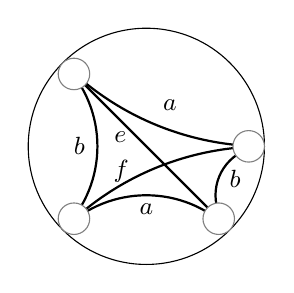
\begin{tikzpicture}
    \tikzset{font=\small}
    \begin{scope}[shift={(0,0)}]
      \draw (0,0) circle (1.5);

      \draw[thick] (315:1.5) arc( 45:135:1.5);
      \draw[thick] (225:1.5) arc(315:405:1.5);

      \draw[thick] (  0:1.5) arc(270:225:3.615);
      \draw[thick] (315:1.5) arc(225: 90:0.622);

      \draw[thick, black] (315:1.5) -- (135:1.5);
      \draw[thick, black] (225:1.5) arc(135: 90:3.617);

      \draw[gray, fill=white] (  0:1.5 - 0.2) circle (0.2);
      \draw[gray, fill=white] (135:1.5 - 0.2) circle (0.2);
      \draw[gray, fill=white] (225:1.5 - 0.2) circle (0.2);
      \draw[gray, fill=white] (315:1.5 - 0.2) circle (0.2);

      \node (l01) at (270:0.80) {$a$};
      \node (l12) at (180:0.85) {$b$};
      \node (l23) at ( 60:0.60) {$a$};
      \node (l30) at (340:1.20) {$b$};
      \node (l02) at (160:0.35) {$e$};
      \node (l02) at (225:0.45) {$f$};
    \end{scope}
  \end{tikzpicture}
\end{document}
